% =====================================================================
%  TP 0 — Fondamentaux de l'ESP32-S3
%  Refonte 2026 (ancienne version : Arduino Due / SAM3X8E)
%
%  Ce chapitre est un document de RÉFÉRENCE : il ne contient pas
%  d'exercices notés. Les questions (T./E.) sont dans les TP 1 et suivants.
%
%  Les blocs "SPOT CODE" indiquent où insérer les liens vers les
%  snippets du dépôt. Les snippets correspondants sont dans
%  tp0/code-snippets/.
% =====================================================================

\chapter{Fondamentaux de l'ESP32-S3}

\section*{Motivation}

L'objectif de ce TP est de revoir les notions d'acquisition sur microcontrôleur vues en Cours 1. Le traitement numérique du signal exige de maîtriser à la fois la fréquence d'échantillonnage et le temps d'exécution.\\

Ce chapitre sert de \textbf{document de référence} pour l'ensemble du module : il ne contient pas d'exercice noté, mais présente la carte, les périphériques que nous utiliserons (GPIO, timers, interruptions, ADC) et surtout la \textbf{façon de les programmer}.\\

C'est ce dernier point qui structure tout le chapitre. Sur une carte comme l'Arduino UNO, il n'existe pratiquement que deux façons de faire : la fonction Arduino, ou le registre. Sur un SoC moderne comme l'ESP32-S3, il en existe \textbf{trois}, et savoir à quel niveau se placer est une compétence d'ingénieur en soi.

\begin{imp}
\textbf{Fil conducteur du TP.} Trois niveaux de programmation coexistent :
\begin{enumerate}
    \item l'\textbf{API Arduino} (Arduino-ESP32) : simple, portable d'une carte à l'autre, mais peu configurable ;
    \item les \textbf{drivers ESP-IDF} : contrôle fin du périphérique, portable entre puces Espressif uniquement ;
    \item l'\textbf{accès direct aux registres} : contrôle total, mais code spécifique à une puce et non réutilisable.
\end{enumerate}
Plus on descend, plus on gagne en contrôle et en performance ; plus on perd en lisibilité, en portabilité et en temps de développement.
\end{imp}

\newpage

% =====================================================================
\section{La carte : ESP32-S3-WROOM-1-N16R8}
% =====================================================================

L'ESP32-S3 est un microcontrôleur 32 bits double c\oe ur Xtensa LX7 cadencé jusqu'à $240\,\mathrm{MHz}$. Le module WROOM-1-N16R8 embarque \textbf{16 Mo de mémoire flash} et \textbf{8 Mo de PSRAM} (mémoire vive externe, à ne pas confondre avec la SRAM interne de la puce, limitée à 512 Ko). Il dispose de capacités Wi-Fi et Bluetooth Low Energy, ainsi que d'un ensemble de périphériques matériels : GPIO, timers, ADC, I2S, SPI et contrôleurs DMA.\\

\begin{imp}
Trois documents de référence à utiliser :
la \href{https://www.mouser.fr/datasheet/3/1574/1/esp32-s3-wroom-1_wroom-1u_datasheet_en.pdf}{datasheet de l'ESP32-S3},
le \href{https://documentation.espressif.com/esp32-s3_technical_reference_manual_en.pdf}{Technical Reference Manual} (TRM),
et la \href{https://docs.espressif.com/projects/arduino-esp32/en/latest/getting_started.html}{documentation Arduino-ESP32}.\\
La datasheet décrit les caractéristiques physiques du composant et le rôle de ses broches ; le TRM détaille l'architecture interne des périphériques et leurs registres ; la documentation Arduino-ESP32 présente les fonctions logicielles et les drivers permettant de les configurer.
\end{imp}

L'ESP32-S3 peut être programmé en \textit{bare-metal}, où le programme pilote directement les ressources matérielles, ou avec un \textit{RTOS} (\textit{Real-Time Operating System}), qui permet notamment de planifier plusieurs tâches. Les frameworks que nous utiliserons reposent tous sur \textbf{FreeRTOS}, qui prend en charge l'ordonnancement des tâches, leur répartition sur les deux c\oe urs, ainsi que les mécanismes de synchronisation et de communication entre elles.\\

\begin{imp}
\textbf{Conséquence pratique.} Même un croquis Arduino minimal tourne à l'intérieur d'une tâche FreeRTOS. Votre \texttt{loop()} n'est pas seule sur la puce : la pile Wi-Fi, le watchdog et le \textit{scheduler} tournent aussi. C'est l'une des raisons pour lesquelles une boucle de \textit{polling} ne peut pas garantir une fréquence d'échantillonnage stable.
\end{imp}

Le kit électronique de l'ECE inclut une \textbf{NeuroBoard-S3}, une variante de l'ESP32-S3 conçue pour faciliter l'intégration d'une caméra (OV3660) et dotée d'une LED multicolore intégrée ($\texttt{RGB\_LED}$). Son brochage est présenté ci-dessous :

\begin{figure}[!h]
\centering
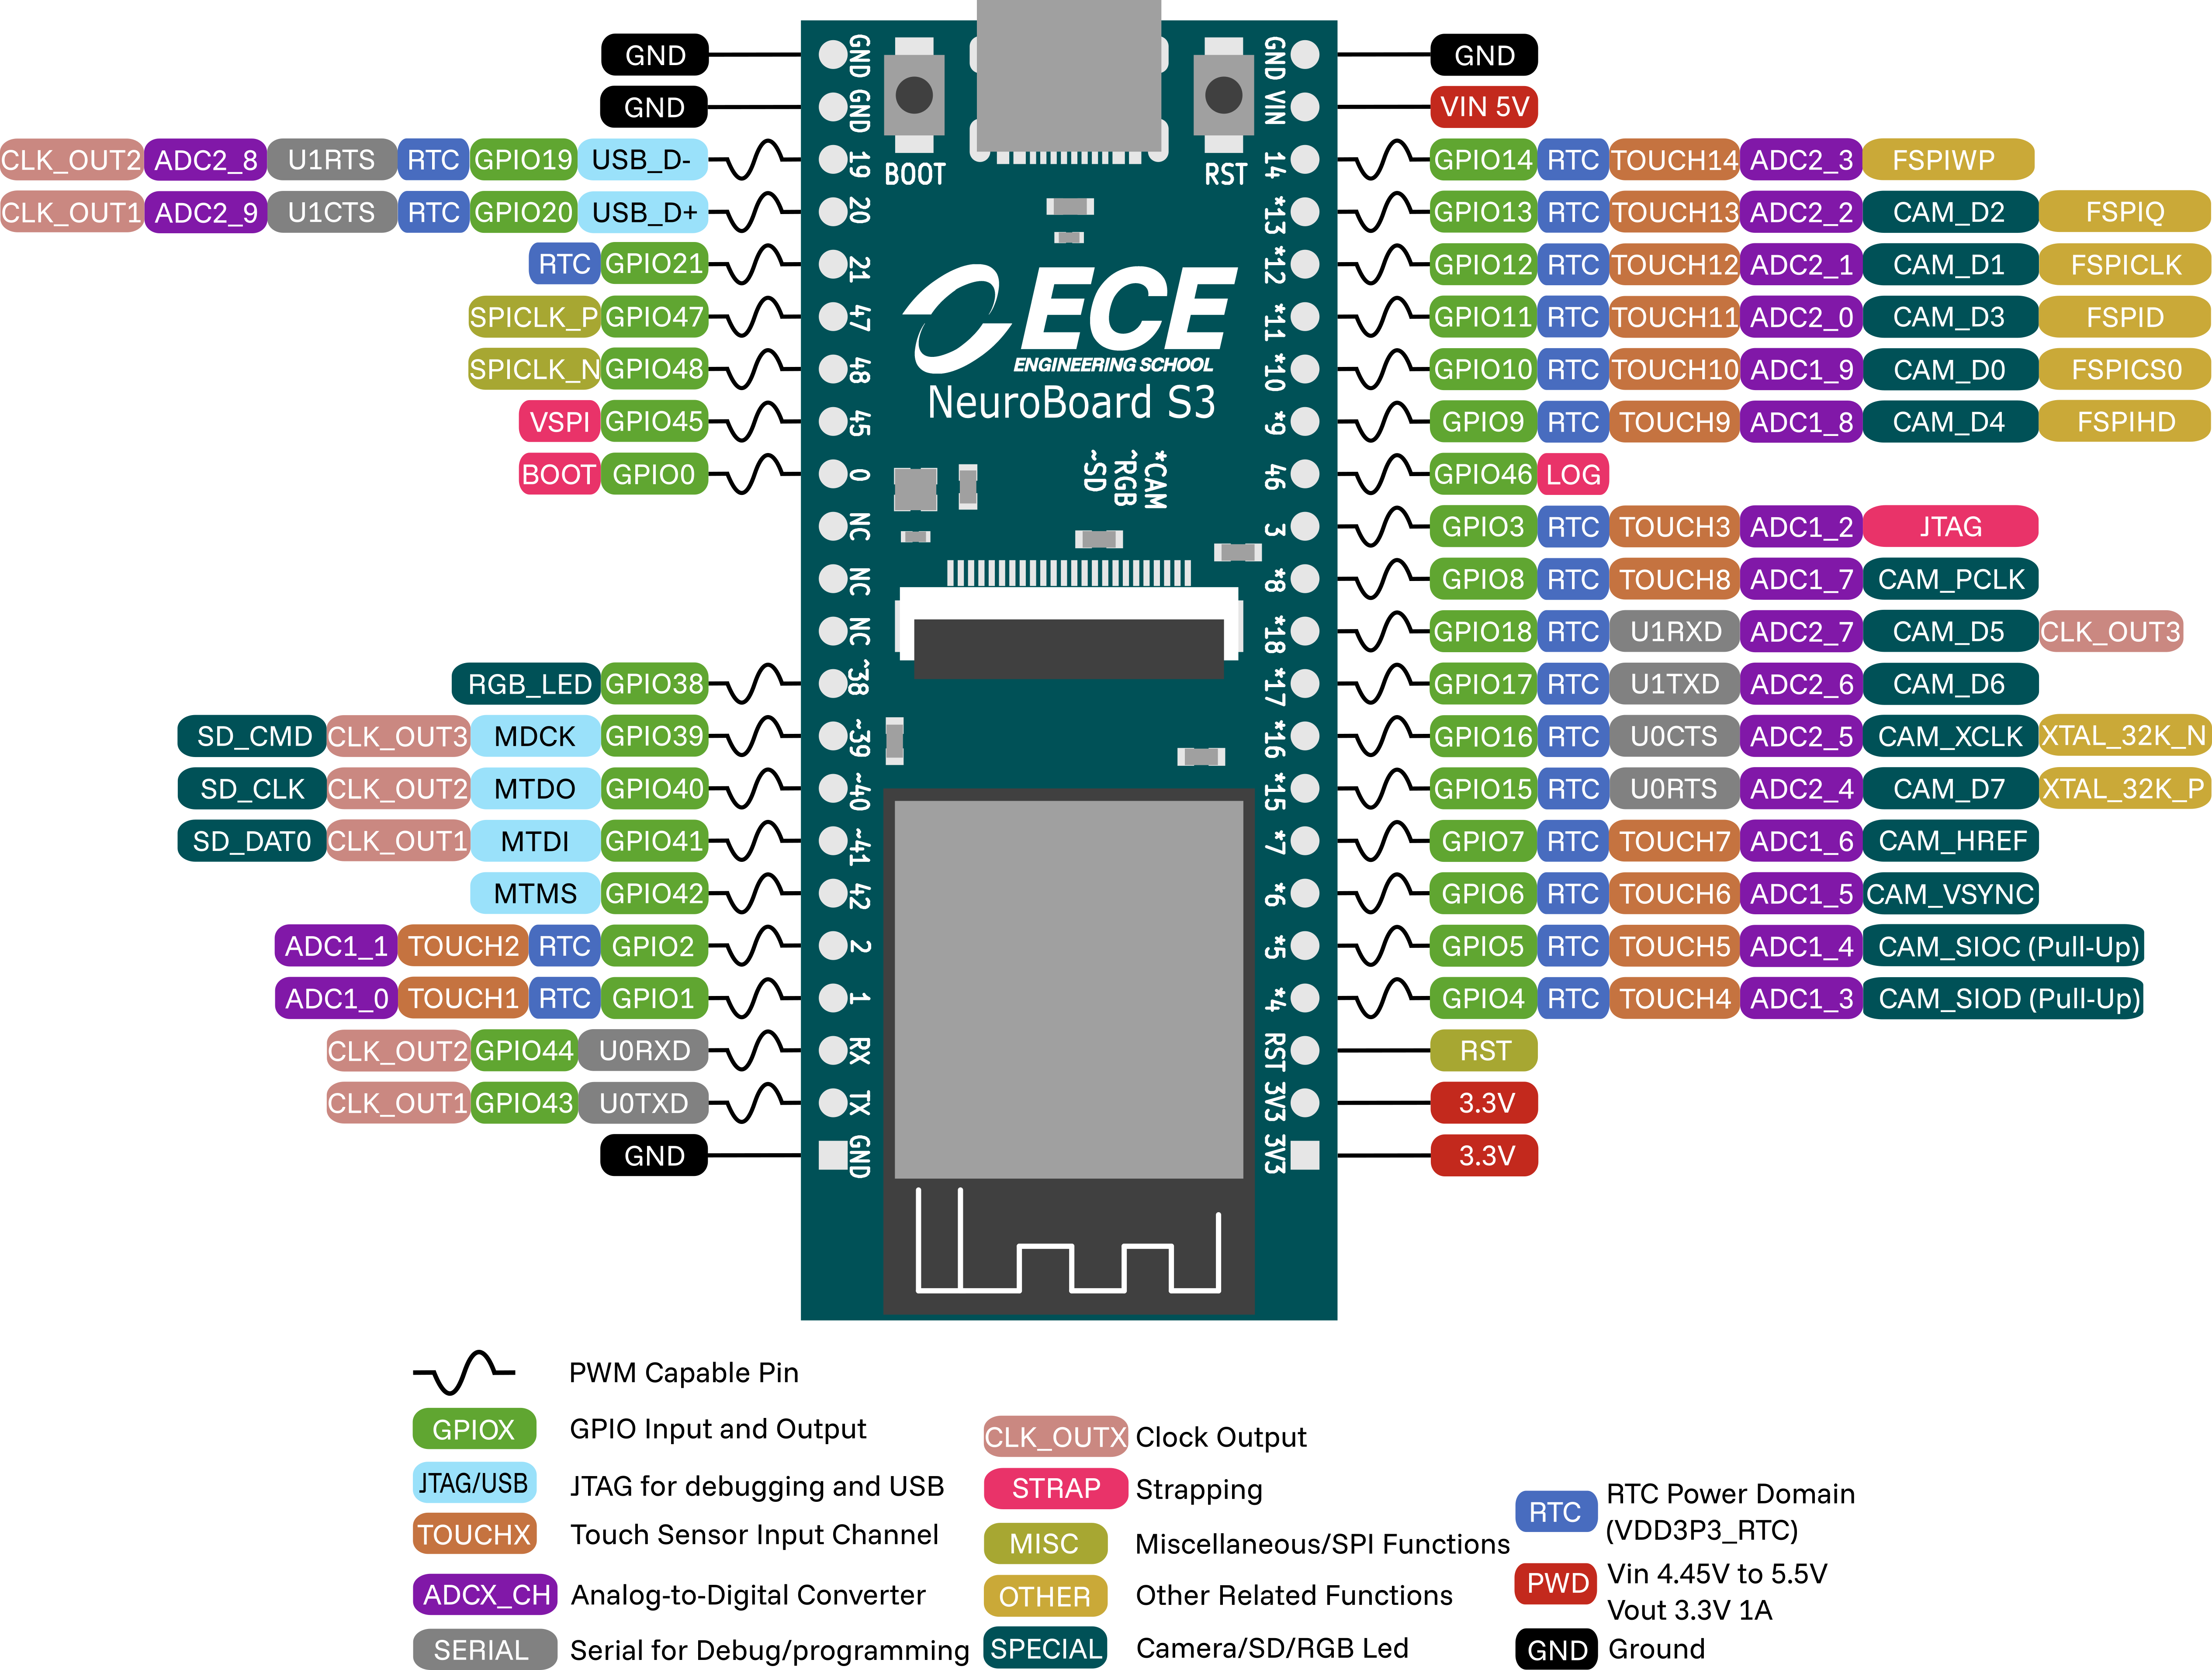
\includegraphics[width=0.7\textwidth]{images/tp0/neuroboard-s3-pinout.png}
\caption{Pinout de la NeuroBoard-S3}
\label{fig:esp32-s3-module-schema}
\end{figure}

\begin{imp}
\textbf{Attention aux broches.} Sur ESP32-S3, la quasi-totalité des GPIO sont routables vers n'importe quel périphérique via la \textit{GPIO matrix}. Trois exceptions à connaître :
\begin{itemize}
    \item les broches \textbf{ADC1} sont figées (GPIO1 à GPIO10) ;
    \item les GPIO 26 à 32 sont utilisées par la flash et la PSRAM : \textbf{ne pas y toucher} ;
    \item la tension maximale d'entrée est de $3{,}3\,\mathrm{V}$. Dépasser cette valeur détruit la puce de manière irréversible.
\end{itemize}
\end{imp}

\newpage

% =====================================================================
\section{Trois niveaux de programmation}
% =====================================================================

\subsection{Arduino-ESP32, ESP-IDF et les registres}

Deux frameworks principaux coexistent pour programmer l'ESP32-S3.\\

\textbf{ESP-IDF} (\textit{Espressif IoT Development Framework}) est le SDK natif et officiel du fabricant. Écrit en C, il offre un contrôle complet sur le silicium, une gestion fine de l'énergie et une intégration native avec FreeRTOS. C'est l'outil de référence pour le développement professionnel et la mise en production, mais sa courbe d'apprentissage est exigeante (configuration CMake, API verbeuses).\\

\textbf{Arduino-ESP32} (\textit{Arduino Core for ESP32}) est une surcouche logicielle construite \textit{par-dessus} ESP-IDF. Son objectif est de rendre la puce accessible via l'API Arduino familière ($\texttt{setup()}$, $\texttt{loop()}$, $\texttt{digitalWrite()}$, etc.). Il est idéal pour le prototypage rapide, car il masque la complexité de la configuration matérielle.\\

Le point important est que ces deux frameworks ne s'excluent pas. Arduino-ESP32 \textit{étant} construit sur ESP-IDF, un croquis Arduino peut appeler directement n'importe quel driver ESP-IDF : il suffit d'inclure l'en-tête correspondant. Et rien n'interdit, dans ce même croquis, d'écrire directement dans un registre.\\

On obtient donc trois niveaux superposés, résumés dans le tableau~\ref{tab:niveaux}.

\begin{table}[!h]
\centering
\renewcommand{\arraystretch}{1.3}
\begin{tabular}{|p{3.1cm}|p{3.4cm}|p{3.4cm}|p{3.4cm}|}
\hline
 & \textbf{API Arduino} & \textbf{Drivers ESP-IDF} & \textbf{Registres} \\
\hline
Exemple (GPIO) & \texttt{digitalWrite()} & \texttt{gpio\_set\_level()} & \texttt{GPIO\_OUT\_W1TS\_REG} \\
\hline
Portabilité & Toute carte Arduino & Puces Espressif & Une seule puce \\
\hline
Contrôle & Faible & Élevé & Total \\
\hline
Lisibilité & Excellente & Correcte & Faible \\
\hline
Documentation & Arduino-ESP32 & ESP-IDF & TRM \\
\hline
\end{tabular}
\caption{Les trois niveaux d'accès au matériel sur ESP32-S3}
\label{tab:niveaux}
\end{table}

\begin{imp}
Il ne s'agit pas de choisir un niveau une fois pour toutes. Un programme bien écrit \textbf{mélange les trois} : Arduino pour l'initialisation et le débogage, ESP-IDF pour les périphériques critiques (timer d'échantillonnage, ADC continu), et les registres uniquement dans les portions où chaque cycle compte, typiquement à l'intérieur d'une ISR.
\end{imp}

\subsection{Un exemple mesurable : faire basculer une broche}

Le meilleur moyen de sentir la différence est de la mesurer. Le croquis ci-dessous fait basculer la même broche $100\,000$ fois, successivement avec les trois approches, et affiche la durée de chaque boucle sur le port série.\\

L'écart n'a rien de théorique : \texttt{digitalWrite()} doit à chaque appel vérifier la validité de la broche, consulter une table de correspondance, gérer le cas où la broche est pilotée par un autre périphérique, puis appeler le driver. L'écriture registre, elle, se réduit à un seul accès mémoire.

% ---------------------------------------------------------------------
% SPOT CODE 1 — comparaison des trois niveaux sur un simple GPIO
% Fichier : tp0/code-snippets/gpio_three_levels.ino
% ---------------------------------------------------------------------
\RepoLink{tp0/code-snippets/gpio_three_levels.ino}{Comparaison des trois niveaux sur un GPIO}

\begin{imp}
\textbf{À retenir :} le gain est réel mais il se paie. La version registre du croquis ne fonctionne que sur ESP32-S3, ne gère pas les GPIO au-delà de 31 (il faut alors utiliser \texttt{GPIO\_OUT1\_W1TS\_REG}), et ne vérifie rien. Ce compromis n'a de sens que si le profilage a montré que ce code est effectivement le goulot d'étranglement.
\end{imp}

\subsection{Rappels de C bas niveau}

Dès que l'on descend au niveau des registres, on manipule des bits. Les opérations bit-à-bit du C sont donc incontournables :

\begin{center}
\begin{tabular}{|c|c|c|c|c|c|}
\hline
AND & OR & XOR & NOT & Décalage gauche & Décalage droite \\
\hline
\texttt{\&} & \texttt{|} & \texttt{\^{}} & \texttt{\~{}} & \texttt{<<} & \texttt{>>} \\
\hline
\end{tabular}
\end{center}

Les trois idiomes à connaître, pour un registre \texttt{REG} et un bit numéro \texttt{n} :

\begin{center}
\begin{tabular}{ll}
Activer un bit  & \texttt{REG |= (1UL << n);} \\
Effacer un bit  & \texttt{REG \&= \~{}(1UL << n);} \\
Tester un bit   & \texttt{if (REG \& (1UL << n)) \{ ... \}} \\
\end{tabular}
\end{center}

Le \texttt{|=} est essentiel : il permet de modifier un bit \textbf{sans écraser} les autres bits du registre, qui configurent souvent d'autres fonctions du même périphérique.\\

Trois mots-clés reviendront en permanence dans la suite du module :

\begin{itemize}
    \item \texttt{volatile} : indique au compilateur que la variable peut être modifiée en dehors du flot normal du programme (par une ISR, ou par le matériel). Sans lui, le compilateur peut optimiser une lecture en la remplaçant par une valeur mise en cache dans un registre du CPU, et le programme ne verra jamais le changement. \textbf{Toute variable partagée entre une ISR et le \texttt{loop()} doit être \texttt{volatile}.}
    \item \texttt{IRAM\_ATTR} : force le placement d'une fonction en RAM interne plutôt qu'en flash. Indispensable pour une ISR, car la flash peut être temporairement inaccessible (opération d'écriture en cours) au moment où l'interruption survient.
    \item les types de taille fixe (\texttt{uint8\_t}, \texttt{uint16\_t}, \texttt{uint32\_t}) : en embarqué on choisit explicitement la taille de ses variables. Un buffer de $4096$ échantillons occupe $8\,\mathrm{Ko}$ en \texttt{uint16\_t} contre $16\,\mathrm{Ko}$ en \texttt{int} — sur 512 Ko de SRAM, cela compte.
\end{itemize}

\begin{imp}
\textbf{Piège classique du 16 bits.} Le produit de deux \texttt{uint16\_t} ne tient pas dans un \texttt{uint16\_t}. Lors d'un filtrage (TP 8), il faut accumuler la convolution dans un \texttt{int32\_t}, puis reconvertir en 16 bits par décalage. Nous y reviendrons.
\end{imp}

\newpage

% =====================================================================
\section{Les interruptions}
% =====================================================================

Une \textbf{interruption} suspend l'exécution du programme principal pour exécuter une fonction dédiée, l'\textit{Interrupt Service Routine} (ISR), puis reprend exactement là où elle s'était arrêtée. C'est le mécanisme qui permet de réagir à un événement matériel sans passer son temps à le surveiller.\\

L'alternative est le \textbf{polling} : interroger l'état de la broche à chaque tour de boucle. Cette approche est simple, mais elle consomme du CPU en permanence et sa réactivité dépend de la durée du reste de la boucle. Si le \texttt{loop()} met $10\,\mathrm{ms}$ à s'exécuter, un appui bref sur un bouton peut passer inaperçu.

\subsection{Deux niveaux, l'exemple de l'Arduino UNO}

La manière de configurer une interruption dépend du niveau auquel on travaille. On peut soit utiliser une \textbf{abstraction} fournie par le framework, soit configurer directement le mécanisme d'interruption \textbf{via les registres}.\\

L'\textbf{API Arduino} masque les détails matériels. La fonction \texttt{attachInterrupt()} associe une fonction à une interruption sans configurer de registre, et \texttt{digitalPinToInterrupt()} convertit le numéro de broche physique en identifiant d'interruption matérielle, ce qui rend le code portable d'une carte à l'autre.\\

Mais le microcontrôleur propose souvent plusieurs mécanismes d'interruption, et l'abstraction n'en expose qu'une partie. L'Arduino UNO, basée sur l'ATmega328P, en est l'illustration la plus nette.

\begin{figure}[!h]
\centering
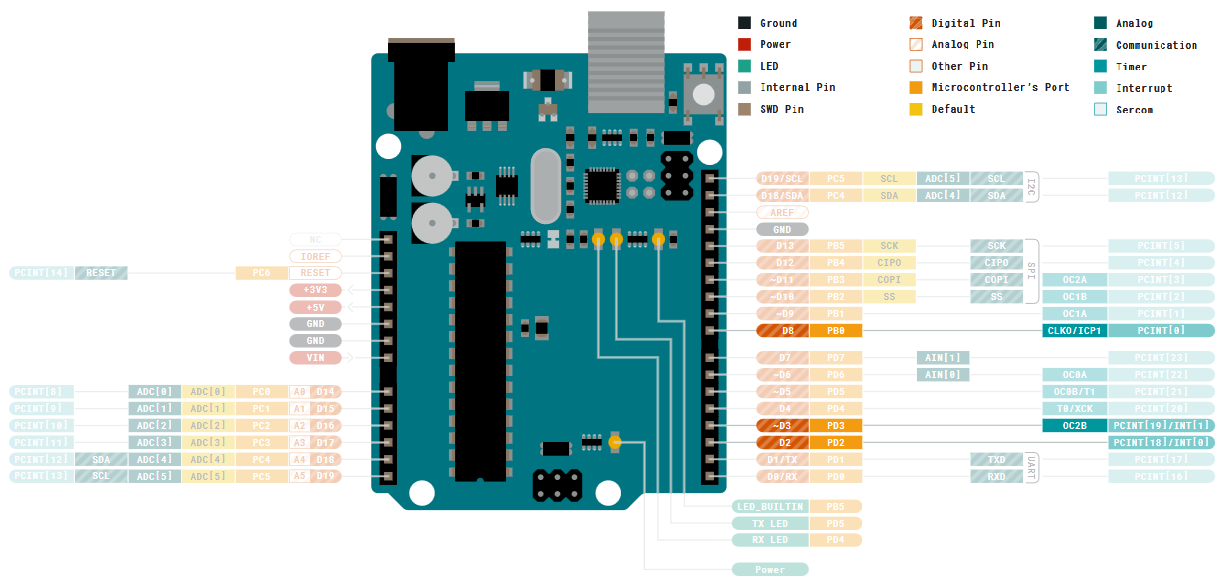
\includegraphics[width=0.9\textwidth]{images/tp0/arduino-pinout.png}
\caption{Pinout de l'Arduino UNO}
\end{figure}

Sur l'ATmega328P, deux mécanismes distincts détectent un changement d'état sur une broche :\\

Les \textbf{interruptions externes} (\texttt{INT0} et \texttt{INT1}) sont associées à deux broches dédiées, les GPIO 2 et 3 sur l'UNO. Elles se configurent finement (front montant, front descendant, niveau bas) et disposent chacune de leur propre vecteur d'interruption. Ce sont celles, et uniquement celles, que \texttt{attachInterrupt()} expose sur l'UNO.\\

Les \textbf{Pin Change Interrupts} (\texttt{PCINT}) reposent sur un autre mécanisme matériel et couvrent un ensemble beaucoup plus large de broches. Le GPIO 8 correspond ainsi à \texttt{PB0}, qui porte la fonction \texttt{PCINT0}. La contrepartie est qu'un seul vecteur d'interruption dessert tout un groupe de broches : l'ISR doit elle-même déterminer quelle broche a changé, et le sens du front n'est pas configurable.\\

\textbf{L'abstraction ne donne donc pas accès à un tiers du matériel disponible.} Pour utiliser une PCINT sur le GPIO 8, il faut ouvrir la datasheet, identifier que le GPIO 8 est \texttt{PB0}, et activer les bits correspondants dans les registres \texttt{PCICR} et \texttt{PCMSK0}. Le code devient spécifique à l'ATmega328P, mais il accède à un mécanisme que \texttt{attachInterrupt()} ne permet pas d'atteindre.

% ---------------------------------------------------------------------
% SPOT CODE 2 — les trois approches sur bouton, cible Arduino UNO
% Fichiers : tp0/code-snippets/button_polling.ino
%            tp0/code-snippets/button_interrupt_arduino.ino
%            tp0/code-snippets/button_interrupt_registers_uno.ino
% ---------------------------------------------------------------------
\RepoLink{tp0/code-snippets/button_polling.ino}{Détection par polling}
\RepoLink{tp0/code-snippets/button_interrupt_arduino.ino}{Détection par interruption, API Arduino}
\RepoLink{tp0/code-snippets/button_interrupt_registers_uno.ino}{Détection par PCINT, registres ATmega328P}

\subsection{Les interruptions GPIO sur ESP32-S3}

Sur ESP32-S3, la contrainte de l'UNO disparaît : \textbf{toutes les broches d'entrée peuvent déclencher une interruption}, et \texttt{attachInterrupt()} fonctionne sur chacune d'elles. L'abstraction est donc beaucoup moins limitante que sur l'UNO.\\

Ce que l'API Arduino ne montre pas, en revanche, c'est ce qu'elle fait pour vous. Sous \texttt{attachInterrupt()} se trouve le driver GPIO d'ESP-IDF, qui installe un service d'interruption partagé (\texttt{gpio\_install\_isr\_service()}), y enregistre un \textit{handler} par broche (\texttt{gpio\_isr\_handler\_add()}) et configure le type de front (\texttt{gpio\_set\_intr\_type()}). Passer au niveau ESP-IDF permet notamment de choisir le c\oe ur sur lequel l'interruption est servie, son niveau de priorité, et de placer l'ISR en IRAM.

\begin{imp}
\textbf{Règles à respecter dans une ISR sur ESP32-S3.} Elles ne sont pas optionnelles : leur violation provoque un \textit{crash} ou un redémarrage par le watchdog.
\begin{itemize}
    \item Une ISR doit être \textbf{courte}. Idéalement : lever un drapeau, incrémenter un compteur, et sortir. Le traitement se fait dans le \texttt{loop()} ou dans une tâche.
    \item Marquer l'ISR \texttt{IRAM\_ATTR}.
    \item \textbf{Pas de \texttt{Serial.print()}, pas de \texttt{delay()}, pas de \texttt{malloc()}} dans une ISR.
    \item Toute variable partagée avec le programme principal doit être \texttt{volatile}.
    \item L'ESP32-S3 étant \textit{dual-core}, \texttt{volatile} ne suffit pas toujours : pour une section critique, utiliser un \texttt{portMUX\_TYPE} avec \texttt{portENTER\_CRITICAL\_ISR()} / \texttt{portEXIT\_CRITICAL\_ISR()}.
\end{itemize}
\end{imp}

Un point pratique enfin : un bouton mécanique \textbf{rebondit}. Un appui unique produit typiquement plusieurs dizaines de transitions en quelques millisecondes, et donc plusieurs dizaines d'interruptions. Un anti-rebond logiciel (comparaison avec \texttt{millis()} dans l'ISR) ou matériel (condensateur) est indispensable — c'est d'ailleurs un défaut que le \textit{polling} masque naturellement, et que l'interruption révèle brutalement.

% ---------------------------------------------------------------------
% SPOT CODE 3 — interruption GPIO sur ESP32-S3, niveaux Arduino et ESP-IDF
% Fichiers : tp0/code-snippets/esp32_button_arduino.ino
%            tp0/code-snippets/esp32_button_idf.ino
%            tp0/code-snippets/esp32_button_registers.ino  (avancé, optionnel)
% ---------------------------------------------------------------------
\RepoLink{tp0/code-snippets/esp32_button_arduino.ino}{Interruption GPIO, API Arduino}
\RepoLink{tp0/code-snippets/esp32_button_idf.ino}{Interruption GPIO, driver ESP-IDF}
\RepoLink{tp0/code-snippets/esp32_button_registers.ino}{Interruption GPIO au niveau registre (avancé)}

\begin{imp}
\textbf{À retenir :} sur ESP32-S3, descendre au niveau registre pour une interruption GPIO n'apporte quasiment rien — le driver ESP-IDF expose déjà tout ce que le matériel sait faire. Le troisième croquis est fourni pour montrer ce que le driver fait réellement, pas comme une pratique à adopter. \textbf{Savoir qu'un niveau existe, c'est aussi savoir quand il est inutile d'y descendre.}
\end{imp}

\newpage

% =====================================================================
\section{Les Timers / Counters}
% =====================================================================

Les \textbf{Timers/Counters} sont des périphériques matériels dédiés au comptage du temps. Contrairement à \texttt{millis()}, qui fournit une mesure du temps lue par le programme, un timer matériel possède son propre compteur qui évolue automatiquement à partir d'une horloge, indépendamment du CPU. Il peut déclencher une \textbf{alarme} lorsqu'une valeur est atteinte, et provoquer une interruption.\\

La différence est décisive pour l'échantillonnage. Une temporisation gérée avec \texttt{millis()} dans une boucle de \textit{polling} dépend de la durée d'exécution des autres instructions de la boucle : l'instant réel de déclenchement dérive et fluctue (\textit{jitter}). Un timer matériel, lui, déclenche exactement à l'échéance programmée, quel que soit ce que fait le CPU par ailleurs. \textbf{C'est la seule façon d'obtenir une fréquence d'échantillonnage $F_e$ digne de ce nom.}

\subsection{Prescaler et résolution}

Le compteur n'avance pas nécessairement à chaque cycle de l'horloge source. Un \textbf{prescaler} divise la fréquence de l'horloge avant qu'elle n'alimente le compteur, ce qui permet de choisir la résolution temporelle adaptée au besoin.\\

Avec une fréquence de comptage de $1\,\mathrm{MHz}$, chaque incrément correspond à $1\,\mu s$ ; une alarme réglée à $1000$ ticks déclenche alors un événement toutes les $1\,\mathrm{ms}$. De manière générale :

\begin{equation}
f_{\text{comptage}} = \frac{f_{\text{source}}}{\text{prescaler}}
\qquad\text{et}\qquad
N_{\text{alarme}} = \frac{f_{\text{comptage}}}{F_e}
\end{equation}

\subsection{Le matériel de l'ESP32-S3}

L'ESP32-S3 contient \textbf{deux groupes de timers}, chacun comportant \textbf{deux timers} génériques, soit \textbf{quatre timers} au total. Ce sont des compteurs \textbf{54 bits} pilotés par des prescalers \textbf{16 bits}, capables de compter vers le haut ou vers le bas, avec rechargement automatique à l'alarme.\\

L'horloge source est sélectionnable : horloge APB ($80\,\mathrm{MHz}$), oscillateur à quartz XTAL ($40\,\mathrm{MHz}$), ou oscillateur RC rapide. Le choix n'est pas anodin : la fréquence APB peut varier si l'on active la gestion dynamique de fréquence (\textit{DFS}), alors que XTAL reste stable — un point à connaître dès qu'on vise une $F_e$ précise.

\begin{imp}
Un compteur 54 bits à $1\,\mathrm{MHz}$ déborde au bout d'environ $570$ ans. Contrairement aux timers 16 bits des petits AVR, le débordement n'est pas une contrainte de conception ici.
\end{imp}

\subsection{Les trois niveaux appliqués au timer}

Avec \textbf{Arduino-ESP32}, la configuration tient en trois lignes : \texttt{timerBegin(1000000)} configure un timer à $1\,\mathrm{MHz}$, \texttt{timerAttachInterrupt()} y associe une ISR, et \texttt{timerAlarm()} fixe le nombre de ticks avant déclenchement ainsi que le rechargement automatique. \cite{arduino_timer}\\

Avec \textbf{ESP-IDF}, le driver \texttt{GPTimer} expose ce que l'API Arduino décide à votre place : source d'horloge, résolution du compteur, sens de comptage, valeur d'alarme, auto-rechargement, priorité et placement de l'interruption. On y associe une \textit{callback} d'alarme, dont la valeur de retour indique à FreeRTOS si un changement de contexte est nécessaire en sortie d'ISR. \cite{esp32s3_gptimer}\\

Le niveau registre n'est volontairement pas traité ici : configurer un timer group à la main demande de manipuler une dizaine de registres (\texttt{TIMGn\_TxCONFIG\_REG}, \texttt{TIMGn\_TxALARMLO\_REG}, \texttt{TIMGn\_TxLOADLO\_REG}, \dots) pour un résultat strictement identique à celui du driver. Le TRM en donne le détail au chapitre \textit{Timer Group}, pour les curieux.

% ---------------------------------------------------------------------
% SPOT CODE 4 — timer périodique, niveaux Arduino et ESP-IDF
% Fichiers : tp0/code-snippets/esp32_timer_arduino.ino
%            tp0/code-snippets/esp32_timer_gptimer.ino
% ---------------------------------------------------------------------
\RepoLink{tp0/code-snippets/esp32_timer_arduino.ino}{Timer périodique, API Arduino}
\RepoLink{tp0/code-snippets/esp32_timer_gptimer.ino}{Timer périodique, driver GPTimer d'ESP-IDF}

Documentation : \href{https://docs.espressif.com/projects/arduino-esp32/en/latest/api/timer.html}{Arduino-ESP32 Timer API} et \href{https://docs.espressif.com/projects/esp-idf/en/latest/esp32s3/api-reference/peripherals/gptimer.html}{ESP-IDF GPTimer}. \cite{arduino_timer,esp32s3_gptimer}

\begin{imp}
\textbf{Méthode de validation.} Pour vérifier qu'un timer tourne à la bonne fréquence, faites basculer une broche dans l'ISR et observez-la à l'oscilloscope : la période mesurée doit valoir le double de la période d'alarme. C'est la méthode que vous utiliserez au TP 1.
\end{imp}

\newpage

% =====================================================================
\section{L'ADC}
% =====================================================================

L'\textbf{ADC} (\textit{Analog-to-Digital Converter}) convertit une tension analogique, par exemple la sortie d'un capteur, en une valeur numérique exploitable par le processeur. C'est l'élément fondamental de toute chaîne d'acquisition.

\subsection{Le matériel de l'ESP32-S3}

L'ESP32-S3 dispose de \textbf{deux ADC} à approximations successives, de résolution \textbf{12 bits} ($4096$ niveaux) :

\begin{itemize}
    \item \textbf{ADC1} : 10 canaux, câblés sur les GPIO 1 à 10 ;
    \item \textbf{ADC2} : 10 canaux, GPIO 11 à 20 — mais \textbf{ADC2 est partagé avec le pilote Wi-Fi}. Dès que le Wi-Fi est actif, ses conversions échouent. \textbf{Utilisez ADC1 par défaut.}
\end{itemize}

La plage de mesure se règle par un \textbf{atténuateur} d'entrée, à choisir en fonction de l'amplitude du signal :

\begin{center}
\begin{tabular}{|l|l|}
\hline
\textbf{Atténuation} & \textbf{Plage utile approximative} \\
\hline
\texttt{ADC\_ATTEN\_DB\_0}  & $0$ -- $950\,\mathrm{mV}$ \\
\texttt{ADC\_ATTEN\_DB\_2\_5} & $0$ -- $1250\,\mathrm{mV}$ \\
\texttt{ADC\_ATTEN\_DB\_6}  & $0$ -- $1750\,\mathrm{mV}$ \\
\texttt{ADC\_ATTEN\_DB\_12} & $0$ -- $3100\,\mathrm{mV}$ \\
\hline
\end{tabular}
\end{center}

\begin{imp}
L'ADC de l'ESP32-S3 n'est ni parfaitement linéaire ni identique d'une puce à l'autre. Une conversion brute n'est donc pas directement une tension. Espressif fournit une API de calibration (\texttt{esp\_adc/adc\_cali.h}) qui exploite les coefficients gravés en \textit{eFuse} pour convertir une valeur brute en millivolts. À utiliser dès qu'une mesure absolue est nécessaire — pour une analyse spectrale, la valeur brute suffit.
\end{imp}

\subsection{Les limites de \texttt{analogRead()}}

L'API Arduino-ESP32 propose la fonction classique \texttt{analogRead(pin)}, d'une simplicité imbattable. Cette simplicité masque cependant deux défauts rédhibitoires pour nos applications.\\

Elle est d'abord \textbf{bloquante} : le CPU attend la fin de la conversion avant de poursuivre. Elle est surtout \textbf{imprécise en cadence} : l'instant réel de chaque échantillon dépend de la durée d'exécution du reste de la boucle, du \textit{scheduler} FreeRTOS et des interruptions de la pile Wi-Fi. Le résultat n'est pas une fréquence d'échantillonnage, mais une suite d'instants irréguliers.\\

Or tout le traitement du signal repose sur l'hypothèse que les échantillons sont \textbf{régulièrement espacés}. Un jitter d'échantillonnage se traduit directement par du bruit et des artefacts dans le spectre : une FFT calculée sur des données acquises par \texttt{analogRead()} en boucle donnera des résultats faux, et ce d'autant plus que la fréquence visée est élevée.\\

Pour du prototypage ou la lecture d'un potentiomètre, \texttt{analogRead()} reste parfaitement adapté. Pour du traitement du signal, il faut passer au niveau suivant.

\subsection{Le mode continu du driver ESP-IDF, et la DMA}

Le driver \textbf{ADC en mode continu} d'ESP-IDF (\texttt{esp\_adc/adc\_continuous.h}) déporte entièrement l'acquisition vers le matériel :

\begin{enumerate}
    \item un \textbf{timer} interne déclenche les conversions à la fréquence configurée, avec une régularité que le logiciel ne peut pas atteindre ;
    \item les résultats sont transférés de l'ADC vers un tampon en SRAM par le contrôleur \textbf{DMA}, sans intervention du CPU pour chaque échantillon ;
    \item le CPU lit les échantillons \textbf{par blocs}, quand cela l'arrange, et consacre le reste de son temps au traitement.
\end{enumerate}

C'est ici qu'intervient la \textbf{DMA} (\textit{Direct Memory Access}), un mécanisme matériel qui déplace des données entre un périphérique et la mémoire sans intervention du CPU une fois le transfert initié.

\begin{imp}
\textbf{On ne configure pas la DMA "toute seule" sur ESP32-S3.} Contrairement au PDC de l'Arduino Due, ni Arduino-ESP32 ni ESP-IDF n'exposent d'API générique de configuration DMA. Celle-ci est encapsulée par les drivers qui en ont besoin : ADC continu, I2S, SPI. Configurer l'ADC continu, \textbf{c'est} configurer la DMA — c'est l'appel à \texttt{adc\_continuous\_new\_handle()} qui réserve les ressources DMA et alloue les tampons. C'est un très bon exemple de ce qu'apporte une abstraction bien conçue : le mécanisme reste, mais il n'a plus besoin d'être piloté à la main.
\end{imp}

\subsubsection{Mise en \oe uvre}

La configuration se déroule en trois étapes, toutes dans \texttt{setup()} :

\begin{enumerate}
    \item \textbf{Allocation des ressources} — \texttt{adc\_continuous\_new\_handle()} : on définit la taille du tampon interne (\texttt{max\_store\_buf\_size}) et celle d'une trame de conversion (\texttt{conv\_frame\_size}), toutes deux en octets.
    \item \textbf{Configuration des canaux} — \texttt{adc\_continuous\_config()} : canaux à échantillonner, résolution, atténuation, et surtout \texttt{sample\_freq\_hz}.
    \item \textbf{Démarrage} — \texttt{adc\_continuous\_start()} : le matériel échantillonne ensuite de façon autonome.
\end{enumerate}

La lecture se fait par \texttt{adc\_continuous\_read()}, qui remplit un tampon d'octets bruts. Ces octets doivent être réinterprétés comme des structures \texttt{adc\_digi\_output\_data\_t} : sur ESP32-S3, le format \texttt{TYPE2} encode dans chaque résultat le numéro d'unité, le numéro de canal et la donnée sur 12 bits.

\begin{imp}
\textbf{Deux contraintes numériques à ne pas oublier.}
\begin{itemize}
    \item Sur ESP32-S3, \texttt{sample\_freq\_hz} doit être compris entre \textbf{611 Hz et 83 333 Hz}. Les $44{,}1$ et $48\,\mathrm{kHz}$ audio sont donc accessibles, mais on est loin d'une acquisition arbitrairement rapide.
    \item \texttt{conv\_frame\_size} doit être un multiple de \texttt{SOC\_ADC\_DIGI\_DATA\_BYTES\_PER\_CONV}, et \texttt{max\_store\_buf\_size} un multiple de \texttt{conv\_frame\_size}. Un handle mal dimensionné échoue à l'initialisation.
\end{itemize}
\end{imp}

% ---------------------------------------------------------------------
% SPOT CODE 5 — acquisition ADC
% Fichiers : tp0/code-snippets/esp32_adc_analogread.ino   (niveau Arduino)
%            tp0/code-snippets/esp32_adc_continuous.ino   (niveau ESP-IDF + DMA)
% ---------------------------------------------------------------------
\RepoLink{tp0/code-snippets/esp32_adc_analogread.ino}{Acquisition simple avec \texttt{analogRead()}}
\RepoLink{tp0/code-snippets/esp32_adc_continuous.ino}{Acquisition continue (ADC + DMA), driver ESP-IDF}

Documentation : \href{https://docs.espressif.com/projects/arduino-esp32/en/latest/api/adc.html}{Arduino-ESP32 ADC API} et \href{https://docs.espressif.com/projects/esp-idf/en/latest/esp32s3/api-reference/peripherals/adc/adc_continuous.html}{ESP-IDF ADC Continuous Mode Driver}. \cite{arduino_adc,esp32s3_adc_continuous}

\begin{imp}
\textbf{À retenir :} pour une acquisition précise et non bloquante, on abandonne \texttt{analogRead()} au profit du driver ADC continu. Le matériel échantillonne à fréquence fixe et transfère les données en mémoire de façon autonome ; le CPU reste disponible pour le traitement. C'est le socle de tous les TP suivants.
\end{imp}

\newpage

% =====================================================================
\section{Visualiser et valider son signal}
% =====================================================================

Un système d'acquisition ne se valide pas en lisant du code, mais en observant des signaux. Trois outils vous accompagneront :

\begin{itemize}
    \item le \textbf{traceur série} de l'IDE Arduino, pour un contrôle qualitatif immédiat de la forme du signal acquis ;
    \item l'\textbf{oscilloscope} et le \textbf{GBF}, pour valider la fréquence réelle d'un timer, mesurer un temps de conversion, ou comparer entrée et sortie ;
    \item \textbf{Audacity}, pour écouter et analyser spectralement un signal enregistré — un tutoriel est disponible sur la page Toolbox de Boostcamp.
\end{itemize}

\begin{imp}
Le débit du port série est très souvent le facteur limitant. À $115\,200$ bauds, on transmet environ $11\,500$ octets par seconde : cela ne suffit pas à envoyer en temps réel un signal échantillonné à $20\,\mathrm{kHz}$ en 16 bits, qui demanderait $40\,000$ octets par seconde. \textbf{Une acquisition qui semble "perdre des échantillons" est très souvent une liaison série saturée, pas un ADC défaillant.} Augmentez le débit, ou acquérez par blocs avant de transmettre.
\end{imp}

% =====================================================================
\section{Récapitulatif}
% =====================================================================

\begin{table}[!h]
\centering
\renewcommand{\arraystretch}{1.3}
\begin{tabular}{|l|p{3.2cm}|p{3.7cm}|p{3.4cm}|}
\hline
\textbf{Fonction} & \textbf{API Arduino} & \textbf{Driver ESP-IDF} & \textbf{Registres} \\
\hline
GPIO & \texttt{digitalWrite()} & \texttt{gpio\_set\_level()} & \texttt{GPIO\_OUT\_W1TS\_REG} \\
\hline
Interruption GPIO & \texttt{attachInterrupt()} & \texttt{gpio\_isr\_handler\_add()} & \texttt{GPIO\_PINn\_REG} \\
\hline
Timer & \texttt{timerBegin()} & \texttt{gptimer\_new\_timer()} & \texttt{TIMGn\_TxCONFIG\_REG} \\
\hline
ADC & \texttt{analogRead()} & \texttt{adc\_continuous\_*} & \texttt{APB\_SARADC\_*} \\
\hline
DMA & --- & implicite dans le driver & \texttt{GDMA\_*} \\
\hline
Sortie analogique & \texttt{ledcWrite()} & \texttt{i2s\_*} & --- \\
\hline
\end{tabular}
\caption{Correspondance des trois niveaux pour les périphériques du module}
\end{table}

\begin{imp}
\textbf{Ce qu'il faut retenir de ce TP.} Il n'existe pas de "bon" niveau dans l'absolu. Il existe un niveau adapté à une contrainte donnée. Dans la suite du module, la règle sera la suivante : \textbf{écrire au niveau le plus haut qui satisfait la contrainte}, et ne descendre que lorsqu'une mesure — pas une intuition — démontre que c'est nécessaire.
\end{imp}